\documentclass{suturo}

\begin{document}
    \maketitle{Vision}{13.05.2017}{}{1}{}{}{}{}

\makeatletter
\newcommand{\chapterauthor}[1]{%
  {\parindent0pt\vspace*{-47pt}%
  \linespread{2.2}\large\begin{flushright}von: #1\end{flushright}%
  \par\nobreak\vspace*{0pt}}
  \@afterheading%
}
\makeatother

\section*{Architektur und Funktion}
\chapterauthor{Alexander Haar}
Das storage\_place-Paket dient zur Ermittlung des Lagerplatzes eines Objekts.

\begin{figure}[!htb]
        \center{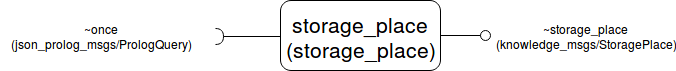
\includegraphics[width=\textwidth]
        {figures/storage_place.png}
        \caption{\label{fig:vision_node} Architektur der storage\_place-node}}
\end{figure}
      
\section*{Methodendokumentation}
\chapterauthor{Alexander Haar}

\subsection{storage\_place}

\subsubsection{createQuery - C++}
\begin{verbatim}
std::string createQuery(std::string object_label)
Beschreibung: Erzeugt eine Prologanfrage, um einen Lagerplatz zu ermitteln.
@param object_label: Der Name des Objekts von dem der Lagerplatz bestimmt werden soll.
\end{verbatim}\label{func:segmentplanes}

\subsubsection{main - C++}
\begin{verbatim}
int main(int argc, char **argv)
Beschreibung: Startet den Knoten.
\end{verbatim}\label{func:findcentergazebo}


\subsubsection{get\_position - Prolog}
\begin{verbatim}
get_position(PositionIndividual, X, Y, Z)
Beschreibung: Extrahiert aus einem Position, die Koordinaten.
@param PositionIndividual: Die Position
@param X: Die X- Koordinate
@param Y: Die Y- Koordinate
@param Z: Die Z- Koordinate
\end{verbatim}\label{func:findposes}

\subsubsection{get\_scale - Prolog}
\begin{verbatim}
get_scale(StorageAreaIndividual, Width, Height)
Beschreibung: Extrahiert aus einer Lagerfläche die Ausmaße.
@param StorageAreaIndividual: Die Lagerfläche
@param Width: Die Breite der Lagerfläche
@param Height: Die Höhe der Lagerfläche
\end{verbatim}\label{func:estimatesurfacenormals}

\subsubsection{storage\_area - Prolog}
\begin{verbatim}
storage_area(ObjectClass, StorageAreaIndividual)
Beschreibung: Ermittelt zu einer Objektklasse die Lagerfläche.
@param ObjectClass: Die Objektklasse zu der eine Lagerfläche ermittelt werden soll.
@param StorageAreaIndividual: Die ermittelte Lagerfläche.
\end{verbatim}\label{func:apply3dfilter}

\subsubsection{storage\_place - Prolog}
\begin{verbatim}
storage_place(ObjectClass, [X, Y, Z], Width, Height)
Beschreibung: Ermittelt zu einer Objektklasse den Lagerplatz.
@param ObjectClass: Die Objektklasse zu der ein Lagerplatz ermittelt werden soll.
@param X: Die X- Koordinate des Lagerplatzes.
@param Y: Die Y- Koordinate des Lagerplatzes.
@param Z: Die Z- Koordinate des Lagerplatzes.
@param Width: Die Breite des Lagerplatzes.
@param Height: Die Höhe des Lagerplatzes.
\end{verbatim}\label{func:estimateplaneindices}

\section*{Schnittstellen}
\chapterauthor{Alexander Haar}

\subsection*{Service Server find\_storage\_place}
\begin{verbatim}
bool find_storage_place(knowledge_msgs::StoragePlace::Request &req,
 knowledge_msgs::StoragePlace::Response &res)
Beschreibung: Service- Methode, welche einen Lagerplatz für Objekte ermittelt.
@param req: Die Anfrage an den Service, welche den Namen des Objekts enthält.  
@param res: Die Antwort des Services, welche das Zentrum und die Ausmaße des Lagerplatzes
            enthält.
@return: true, falls der Aufruf erfolgreich war und false sonst.
\end{verbatim}\label{func:findcluster}

\section*{Programmablauf}
\chapterauthor{Alexander Haar}
\subsection*{Schritt 1: Anfrage an den Service- Server}
Eine Objektklasse wird an den Service- Server übergeben.
\subsection*{Schritt 2: Erstellen der Prologanfrage}
Anhand der Objektklasse wird eine Prologanfrage erstellt und an den json\_prolog- Server geschickt.
\subsection*{Schritt 3: Ermitteln des Lagerplatzes} 
Durch die oben definierten Prologregeln wird unter Verwendung von only- restrictions der Lagerplatz ermittelt.

\subsection*{Schritt 4: Zurückgeben der Antwort}
Die vom json\_prolog- Server erhaltene Antwort wird entsprechend geparst und zurückgegeben.

\end{document}
